\documentclass[useAMS,usenatbib]{mn2e}

\addtolength\topmargin{-2cm}

\pdfoutput=1
\usepackage[varg]{txfonts}
\usepackage{astrojournals}
\usepackage{graphicx}
\usepackage{microtype}
\usepackage{xcolor}
\usepackage{fixltx2e}
\usepackage{hyperref}
\usepackage{siunitx}
\usepackage{xspace}
\hypersetup{colorlinks=True, linkcolor=blue!50!black, citecolor=black,
  urlcolor=blue!50!black}

\usepackage{color}

%%Units
%\newcommand{\degr}{$^\circ$\xspace}

%Solar amounts
\newcommand{\ro}{R$_\odot$\xspace}
\newcommand{\mo}{M$_\odot$\xspace}
\newcommand{\zo}{Z$_\odot$\xspace}

\newcommand{\tc}{$\mathrm{\theta}^1\mathrm{C}$\xspace}

%Physical variables
\newcommand{\teff}{$\mathrm{T}_{\mathrm{eff}}$\xspace}
\newcommand{\te}{$\mathrm{T}_{\mathrm{e}}$\xspace}
\newcommand{\nelec}{$\mathrm{n}_{\mathrm{e}}$\xspace}

%This is necesary for the \ion command works
\DeclareRobustCommand\ion[2]{%
  \mbox{#1\kern0.2em%
    \smaller\rmfamily%
    \edef\@tempa{\@car#2\@nil}%
    \ifcat1\@tempa%
    \@Roman{#2}%
    \else%
    \uppercase{#2}%
    \fi}}
\newcounter{IonStage}
\DeclareRobustCommand\plainion[2]{\setcounter{IonStage}{#2}#1
  \Roman{IonStage}}
\DeclareRobustCommand\nodata{$\cdots$}
\newcommand{\smaller}{\small}

%This are my most used lines
\newcommand{\ha}{H$\alpha$\xspace}
\newcommand{\hb}{H$\beta$\xspace}
\newcommand{\hii}{\ion{H}{ii}\xspace}
\newcommand{\he}{\ion{He}{i}\xspace}
\newcommand{\sii}{[\ion{S}{ii}]\xspace}
\newcommand{\siip}{[\ion{S}{ii}]+\xspace}
\newcommand{\nii}{[\ion{N}{II}]\xspace}
\newcommand{\oi}{[\ion{O}{I}]\xspace}
\newcommand{\oii}{[\ion{O}{II}]\xspace}
\newcommand{\oiii}{[\ion{O}{III}]\xspace}
\newcommand{\neii}{[\ion{Ne}{II}]\xspace}
\newcommand{\lhe}{\ion{He}{I}$\lambda5876$\xspace}
\newcommand{\lsii}{[\ion{S}{II}]$\lambda6716$\xspace}
\newcommand{\lsiimas}{[\ion{S}{II}]$\lambda6716+\lambda6731$\xspace}
\newcommand{\lnii}{[\ion{N}{II}]$\lambda6583$\xspace}
\newcommand{\loi}{[\ion{O}{I}]$\lambda6300$\xspace}
\newcommand{\loii}{[\ion{O}{II}]$\lambda3727$\xspace}
\newcommand{\loiii}{[\ion{O}{III}]$\lambda5007$\xspace}

\newcommand{\R}{$\mathrm{R}$\xspace}

%-------------------------------------------------------
\title[Semi 3D Photoionization with Hydrodynamics for the Proplyds in Orion]{Semi 3D Photoionization with Hydrodynamics for the Proplyds in Orion}
\author[N. Flores-Fajardo and W. Henney]{N. Flores-Fajardo$^{1,2}$\thanks{E-mail:
nahieflores@gmail.com} and W. Henney$^{2}$\thanks{E-mail:
w.henney@gmail.com.}\\
$^{1}$Kavli Institute of Astronomy and Astrophysics, Peking University, China\\
$^{2}$Centro de Radioastronomía y Astrofisica, Universidad Nacional Autonoma de Mexico, Morelia, Mexico.}
%-------------------------------------------------------


\begin{document}

%
%  These Macros are taken from the AAS TeX macro package version 4.0.
%  Include this file in your LaTeX source only if you are not using
%  the AAS TeX macro package and need to resolve the macro definitions
%  in the BibTeX entries returned by the ADS abstract service.
%
%  For more information on the AASTeX macro package, please see the URL
%	http://www.ferberts.com/AAS/aastex.html
%  For more information about ADS abstract server, please see the URL
%	http://adswww.harvard.edu/ads_abstracts.html
%

% Abbreviations for journals.  The object here is to provide authors
% with convenient shorthands for the most "popular" (often-cited)
% journals; the author can use these markup tags without being concerned
% about the exact form of the journal abbreviation, or its formatting.
% It is up to the keeper of the macros to make sure the macros expand
% to the proper text.  If macro package writers agree to all use the
% same TeX command name, authors only have to remember one thing, and
% the style file will take care of editorial preferences.  This also
% applies when a single journal decides to revamp its abbreviating
% scheme, as happened with the ApJ (Abt 1991).

\def\aj{\rm{Astronomical Journal}}                   % Astronomical Journal
\def\araa{\rm{ARA\&A}}             % Annual Review of Astron and Astrophys
\def\apj{\rm{Astrophysical Journal}}                 % Astrophysical Journal
\def\apjl{\rm{Astrophysical Journal, Letters}}                % Astrophysical Journal, Letters
\def\apjs{\rm{Astrophysical Journal, Supplement}}               % Astrophysical Journal, Supplement
\def\ao{\rm{Appl.~Opt.}}           % Applied Optics
\def\apss{\rm{Ap\&SS}}             % Astrophysics and Space Science
\def\aap{\rm{Astronomy and Astrophysics}}                % Astronomy and Astrophysics
\def\aapr{\rm{Astronomy and Astrophysics Reviews}}          % Astronomy and Astrophysics Reviews
\def\aaps{\rm{Astronomy and Astrophysics, Supplement}}              % Astronomy and Astrophysics, Supplement
\def\azh{\rm{AZh}}                 % Astronomicheskii Zhurnal
\def\baas{\rm{BAAS}}               % Bulletin of the AAS
\def\jrasc{\rm{JRASC}}             % Journal of the RAS of Canada
\def\memras{\rm{MmRAS}}            % Memoirs of the RAS
\def\mnras{\rm{Monthly Notices of the RAS}}             % Monthly Notices of the RAS
\def\pra{\rm{Phys.~Rev.~A}}        % Physical Review A: General Physics
\def\prb{\rm{Phys.~Rev.~B}}        % Physical Review B: Solid State
\def\prc{\rm{Phys.~Rev.~C}}        % Physical Review C
\def\prd{\rm{Phys.~Rev.~D}}        % Physical Review D
\def\pre{\rm{Phys.~Rev.~E}}        % Physical Review E
\def\prl{\rm{Phys.~Rev.~Lett.}}    % Physical Review Letters
\def\pasp{\rm{Publications of the ASP}}               % Publications of the ASP
\def\pasj{\rm{PASJ}}               % Publications of the ASJ
\def\qjras{\rm{QJRAS}}             % Quarterly Journal of the RAS
\def\skytel{\rm{S\&T}}             % Sky and Telescope
\def\solphys{\rm{Sol.~Phys.}}      % Solar Physics
\def\sovast{\rm{Soviet~Ast.}}      % Soviet Astronomy
\def\ssr{\rm{Space~Sci.~Rev.}}     % Space Science Reviews
\def\rmxaa{\rm{Rev.Mex. de Astronomia y Astrofisica}}    
\def\zap{\rm{ZAp}}                 % Zeitschrift fuer Astrophysik
\def\nat{\rm{Nature}}              % Nature
\def\iaucirc{\rm{IAU~Circ.}}       % IAU Cirulars
\def\aplett{\rm{Astrophys.~Lett.}} % Astrophysics Letters
\def\apspr{\rm{Astrophys.~Space~Phys.~Res.}}
                % Astrophysics Space Physics Research
\def\bain{\rm{Bull.~Astron.~Inst.~Netherlands}} 
                % Bulletin Astronomical Institute of the Netherlands
\def\fcp{\rm{Fund.~Cosmic~Phys.}}  % Fundamental Cosmic Physics
\def\gca{\rm{Geochim.~Cosmochim.~Acta}}   % Geochimica Cosmochimica Acta
\def\grl{\rm{Geophys.~Res.~Lett.}} % Geophysics Research Letters
\def\jcp{\rm{J.~Chem.~Phys.}}      % Journal of Chemical Physics
\def\jgr{\rm{J.~Geophys.~Res.}}    % Journal of Geophysics Research
\def\jqsrt{\rm{J.~Quant.~Spec.~Radiat.~Transf.}}
                % Journal of Quantitiative Spectroscopy and Radiative Trasfer
\def\memsai{\rm{Mem.~Soc.~Astron.~Italiana}}
                % Mem. Societa Astronomica Italiana
\def\nphysa{\rm{Nucl.~Phys.~A}}   % Nuclear Physics A
\def\physrep{\rm{Phys.~Rep.}}   % Physics Reports
\def\physscr{\rm{Phys.~Scr}}   % Physica Scripta
\def\planss{\rm{Planet.~Space~Sci.}}   % Planetary Space Science
\def\procspie{\rm{Proc.~SPIE}}   % Proceedings of the SPIE

\let\astap=\aap
\let\apjlett=\apjl
\let\apjsupp=\apjs
\let\applopt=\ao



\date{Accepted 1988 December 15. Received 1988 December 14; in original form 1988 October 11}

%\pagerange{\pageref{firstpage}--\pageref{lastpage}} \pubyear{2002}

\maketitle

\label{firstpage}

%--------------------------------------------------------
\begin{abstract}
We present semi 3D models for both, the fully ionized and the partially ionized zones. These models take, for the first time, into account the radiative transfer and the hydrodynamics of the gas flow.
\end{abstract}
%--------------------------------------------------------

\begin{keywords}
Protoplanetary discs, stars: protostars, ISM: abundances, H II regions, ISM individual objects: Orion nebula.
\end{keywords}

%--------------------------------------------------------
\section{Introduction}
\label{sec:introduction}
%--------------------------------------------------------

The Proplyds in the Orion Nebula were discovered as six knots compact emission lines located very close to the high-mass stars of the Trapezium \citep{1979AA.7397L}. Later observations, particularly those of Hubble Space Telescope in direct imaging of emission lines \citep{1993ApJ410..696O,1998AJ....115..263O,1998AJ....116.1346O} have allowed a clear picture of these objects: are accretion disks around young low-mass stars, which are being evaporated by ultraviolet radiation from of a nearby massive star \citep{1998ApJ499..758J, 1998AJ....116..322H, 1999ApJ515..669S}.

\citep{1999AJ....118.2350H} have the photoevaporating models. Fig 5.

Until today, there has not been a comprehensive study of the abundance of heavy elements in the gas phase of any of these objects, even when found evidence of the evolution of dust properties in proplyd's molecular opaque disks \citep{2003ApJ587L.109S} and in the photoevaporated and ionized flow \citep{2001ApJ...561..830G}.

The models developed in this research are semi 3-D models using the 1D photoionization code {\sc CLOUDY} \citep{1998PASP..110..761F} which makes a detailed calculation of radiative transfer. The hydrodynamic of the gas in these models is being taken into account from the introduction of the density and velocity profiles calculated from self-consistent manner the conservation of mass and momentum. Both profiles are specified for both the photoionized zone as well as the ionization front, based on analytical models of W. Henney et al. \citep{1999AJ....118.2350H,2005ApJ...621..328H}.

For the low mass stars in the Orion Nebula, the external radiation field \tc is much more efficient than the internal one in the photoevaporation of the acretion disk. In this case we have:

\begin{itemize}
\item{Far Ultraviolet flux ($6 \, {\rm eV} \, < \, h \nu \, < \, 13.6 \, {\rm eV}$): This flux photodissociates molecules and heat the gas to $100 - 1000 \, {\rm K}$ and it produce a heated thermic neutral wind.} 
\item{Extreme Ultraviolet flux ($13.6 \, {\rm eV} \, < \, h \nu$): This radiation ionized the gas and grows the gas temperature to $\sim 10^4 \, {\rm K}$ and it produce a photoevaporated ionized flux.}
\end{itemize}

%--------------------------------------------------------
\section{Model}
\label{sec:model}
%--------------------------------------------------------

We follow the analytic model of a photoevaporated wind described in \citet{1998AJ....116..322H}.
 
The simplest assumpion is that there is a static semi-spherical distribution of gas around the central low mass star. This gas is being evaporated and ionizing by the radiation coming from \tc

\begin{itemize}
\item{Ionizing radiation incident from only one direction.}
\item{Assuming a cylindrical geometry with symmetry in the coordinate $\Phi$}
\item{Semi-spheric ionization front. $S_{\theta} \, = \, S_0 (cos \, \theta)$}
\item{The photoionized gas flows radially from the border of ionization}
\item{The gas flow is not isotermic}
\end{itemize}

We construct 1D Cloudy models of a series of individual radial cuts from the center of the proplyd, at different angles $\theta$ from the proplyd axis. From these models, we interpolate the physical conditions to create a semi-3D model assuming symmetry in the $\phi$ angle.

\begin{figure}
\centering
  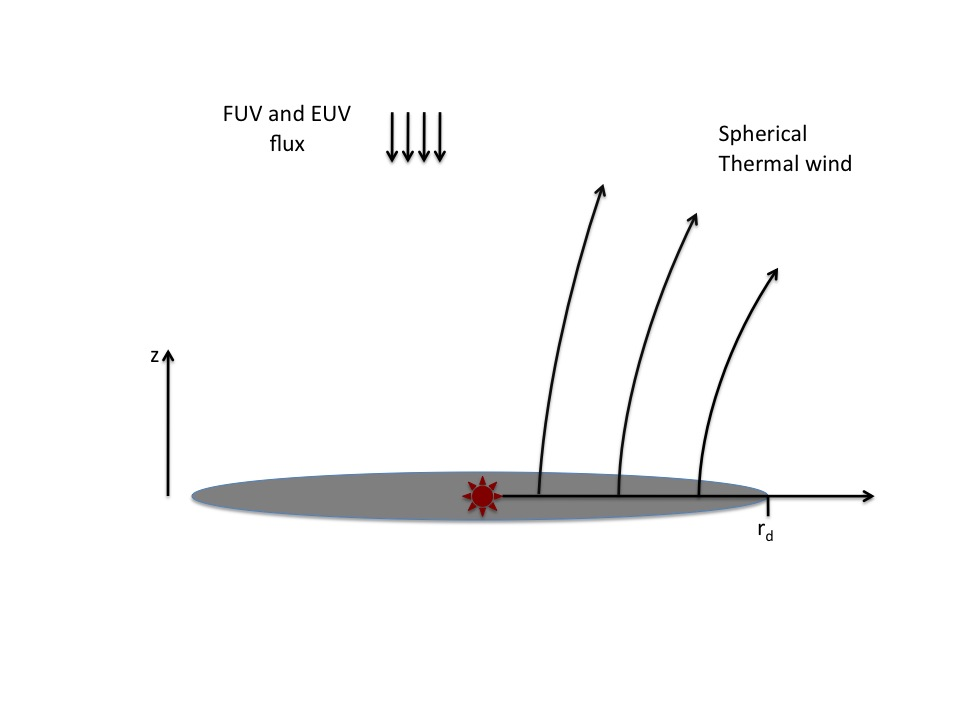
\includegraphics[width=8.5 cm]{viento.jpg}
  \caption{A sketched disk photoevaporation wind.} \label{fig:wind}
\end{figure}

We supose that the disk conditions and physical properties does not change significantly in the $r$ direction. Due that the thermal wind will be only in the $z$ direction, and for those, the ionic structure will be only in the $z$ direction.

%--------------------------------------------------------
\subsection{Geometry}
\label{sec:geometry}
%--------------------------------------------------------

Unlike \hii regions, in the case of disk photoevaporation the geometry is open, in the sense that the ionization front does not enclose the ionized gas. One characteristic of this geometry is that the gas will accelerate when crossing the ionization front, and this will be expand too.
Following the Henney et al. model we consider a critical ``R type'' expansion. This expansion is distinguished by a subsonical flow in the neutral part and a supersonical flow in the ionized part (velocity gas exactly or just a little high than the sonic velocity). It produce a ionization front with small changes in the gas density.

$\Delta$ is the ionization front width in terms of the mean free path at 1 Rydberg. That is, $\Delta \, = \, W \, / \, n_0 \, \sigma_0$ where $n_0$ is the density at the sonic point, $\sigma_0$ is the Hydrogen cross section and $W$ is the number of the mean free paths.

For simplicity and clarity of the model we chose to use a dimenssionless radial coordinate $R \,=\, r\,/\,r_0$ where $r$ is the radial coordinate in $\rm cm$ starting in the low-mass star inside the proplyd and $\rm r_0$ is the distance between the proplyd center, the low-mass star, and the sonic point.

\begin{figure}
\centering
  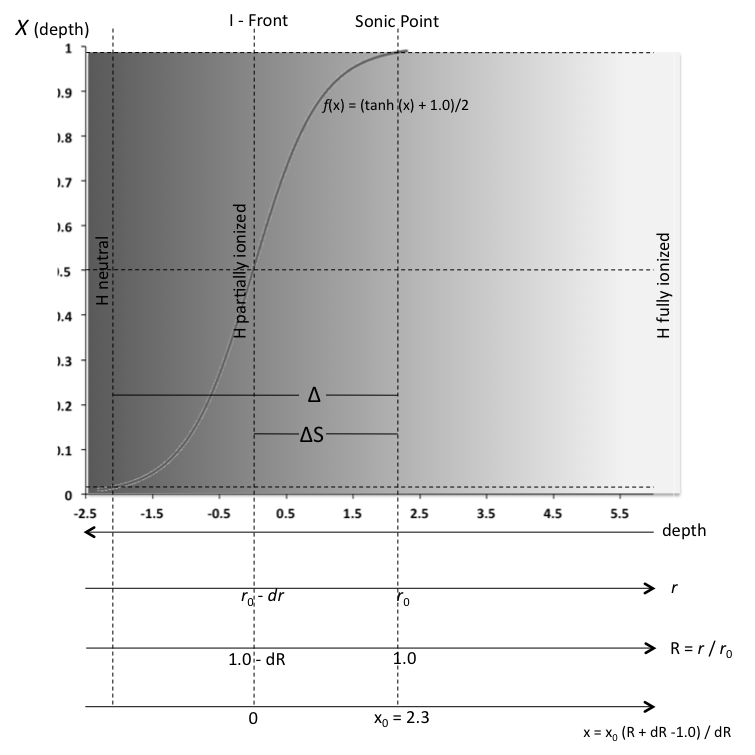
\includegraphics[width=8.5 cm]{./IFront/ifront.png}
  \caption{A sketched geometry of the 1D Cloudy model.} \label{fig:1Dgeom}
\end{figure}

\begin{figure}
  \centering
  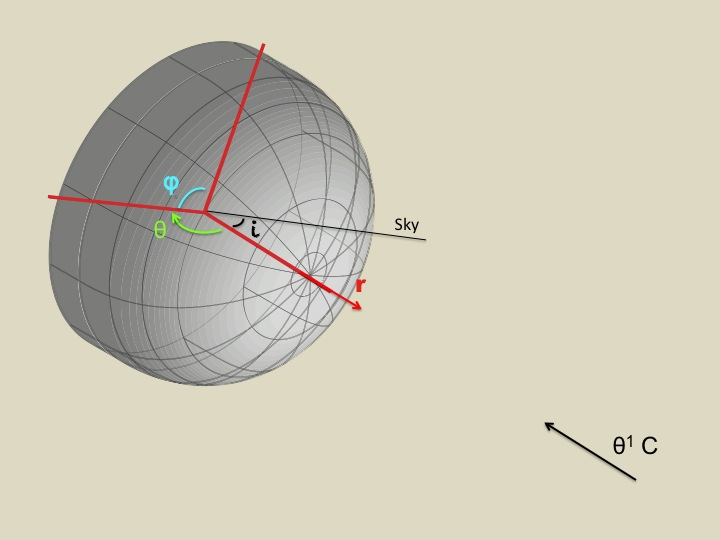
\includegraphics[width=8.5 cm]{./graf_model_3D/geometry_model.jpg}
  \caption{A sketched geometry of the semi-3D model.} \label{fig:3Dgeom}
\end{figure}

%--------------------------------------------------------
\subsection{Radiation field}
\label{sec:radiation}
%--------------------------------------------------------

Due that the proplyds cusp is the only part that is directly exposed to the radiation field of \tc this is the brigthest part of the proplyd at least in \ha and ions of high and medium ionization. The diffuse radiation of the nebulae is negligible in comparation with the \tc in the cusp at least for those proplyds that are very close to \tc, nevertheless we take it into account as a fraction of the main radiation field.

\begin{itemize}
\item{Direct radiation field: The \tc flux that reach the proplyd is $S_0 \, = \, Q_H \, / 4\pi \, D^2$. $Q_H$ is the number of H ionizing photons, and $D$ is the physical distance between \tc and the proplyd. Due that the model is constructed based on  a 1D code, the only part of the radiation that we take into account is that is radial to the Ionization Front in each point, it means, $S'_0 \, = \, S_0 \, cos \theta$. From the ionization equilibrium, $S_0 \sim n_0^2 r_0$, we can find the density at the ionization fron
    \begin{equation}
      n_0 = \left( \frac{S_0}{r_0} \, cos \theta \right) ^{1/2}
    \end{equation}
}
so the greater peak density is for $\theta \, = \, 0$
\item{Diffuse radiation field: This is introduced to the models as constant:
    \begin{equation}
      D_\beta = \frac{1}{4} \frac{\alpha_1}{\alpha_B} \frac{\sigma_{star}}{\sigma_{diffuse}}
    \end{equation}
    where $\alpha_1$ and $\alpha_B$ are the recombination coefficients to the ground level and to the case B respectively.  $\sigma_{star}$ and $\sigma_{diffuse}$ are the star and diffuse radiation field mean effective cross section respectively. $D_\beta \, = \, 0.004$ means that $\sigma_{star} \, = \, 2.5 \, \sigma_{diffuse}$ that is likely for those proplyds nearest to \tc. For those in the outer zones of the nebulae (where the diffuse radiation field is more important) the $D_\beta \, \sim \, 0.1$ \citep{1999AJ....118.2350H}.
}
\end{itemize}

The total radiation field that we consider for the proplyd ionization is: 

\begin{equation}
  S'_0 = S_0 (cos \theta \, + \, D_\beta)
\end{equation}

In this first step of the model we contructed a model for only the proplyd cusp with the influence of the main radiation field, \tc, and the diffuse radiation as a \tc fraction.

%-------------------------------------------------------
\subsection{Radial Density Structure}
\label{sec:density}
%-------------------------------------------------------

As we mentioned above one way to develope models that take into account both, the radiative transfer and the hydrodinamics of the gas, is to introduce an aproximate hydrodinamics in the radiative models that are availables and such are stables. This is our case and the way to introduce the hydrodinamic of the gas is using the electron density structure that is a result of the hydrodinamic teorical models.

We divide the proplyd flow into two zones:

\begin{itemize}
  \item{$\rm r > r_0$: An outer, fully ionized supersonic flow.}
    \item{$\rm r < r_0$: An inner, partially ionized subsonic flow.}
\end{itemize}

This is equivalent to say that the behavior of the physical conditions are diferent in both zones. We suppose that the flow in the partially ionized zone, that correspond to the thin ionization front, is a subsonic flow that is acelerated to be supersonic in the outer fully ionized zone. The boundary between them are exactly the sonic point. The conditions there, and in every point of the proplyd, are fixed by continuity, it means that the electron density change as the gas-phase velocity change and visceversa. 


%-------------------------------------------------------
\subsubsection{The outer fully ionized zone}
\label{sec:outer}
%-------------------------------------------------------

This is similar to what Will did in \citep{2002ApJ...566..315H}

In the outer zone we assume an isothermal, supersonic, complite ionized flow. From mass conservation, in spherical geometry and in the steady state, the radial gas velocity is given by Dyson solution \citep{1968Ap26SS...2..461D}.

\begin{equation}
  R = U^{(-1/2)} exp \left [ \frac{1}{4} \left (U^2 -1 \right )
  \right ]
\end{equation}

where $U(R) = u(R) / c_0$ where $u(R)$ is the gas velocity and $c_0$ is the sound speed. Due that, the analytic solution for $U$ as a function of $R$ is not possible, from this equation generate a table of values for $U$ and $R$ and interpolate this table for each $R$ that is necesary in the Cloudy model.

At each point the density is calculated by the continuity equation:

\begin{equation}
  \rho (R) = \rho (R_{max}) \left ( \frac{U(R_{max})}{U (R)} \right )
    \left ( \frac{R_{max}}{R} \right ) ^2
\end{equation}

%-------------------------------------------------------
\subsubsection{The boundary}
\label{sec:boundary}
%-------------------------------------------------------

Because the gas velocity is the property that determines the behavior of other physical properties of the proplyd, the logical boundary between the regions is exactly the sonic point.

This point is also where the criterion of Stromgren for a density bounded region is met. That is, where the photoionization balance is broken 

\begin{equation}
  N_{H^0} \displaystyle\int_{\nu_0}^{\infty} \frac{4 \, \pi \, J_\nu}{h \, \nu} a_\nu(H^0) d\nu = N_e \, N_p \alpha_B(H^0, \, T)
\end{equation}

and the recombination start to overcome the photoinization.

\begin{equation}
  \rho(R=1) \, = \, \rho(R_{max}) \, U(R_{max}) \, R^2_{max}
\end{equation}

$\rm r = r_0$
$\rm X_H \simeq 0.99$; $X_H$ is the hydrogen ionization fraction
$u = c_0$ by definition of the boundary

%-------------------------------------------------------
\subsubsection{The inner partially ionized zone}
\label{sec:inner}
%-------------------------------------------------------

Partially ionized region: Density is function of sound speed

In this zone, we follow the simplified analytic model for weak--D ionization front described in Appendix of \citet{2005ApJ...621..328H}. Even when this model is for a plane-parallel ionization front (the momentum conservation assumes plane parallel geometry) and this is not our case (we have an divergent geometry) this is an aproximation that could give us a good idea of the advection effects on the I-front.

Following the A8 equation, 
\begin{equation}
  c(X) = c_0 \left [ \frac{T(X)}{T_0} \frac{1+X}{1+X_0}\right]^{1/2}
\end{equation}
If we see the electronic temperature behavior for the weak--D solutions, Fig.18 from \citet{2005ApJ...621..328H}, we can see that the temperature could be assume constant in first aproximation, at least in $0.25 \le X \le 1.0$. This is our case in the inner zone, then the sound speed will be:
\begin{equation}
  c(X) = c_0 \left [ \frac{1+X}{1+X_0}\right]^{1/2}
\end{equation}

As in the Cloudy models the ionization fraction is one of the physical quantities that are calculated in each zone, we can not use it for calculate the sound speed in each zone. Then, we made an aproximation for the behavior of $X$ in the recombination zone, 

\begin{equation}
  X_H = 0.5 (tan h (x) + 1.0)
\end{equation}

where 

\begin{equation}
  x = x_0 \frac{R + dR -1.0}{dR}
\end{equation}

$x_0$ is where the H ionization fraction is 0.99, i.e. the sonic point where $R = 1$.

Making use of the Mach number $M = u/c$ and the fact of $c_0/c = \frac{1}{2} \left ( M + M^{-1} \right)$. Then, once more by continuity, the electronic density in this zone is:
\begin{equation}
  \rho (X) = \rho_0 / \left ( 1.0 - \sqrt{ 1.0 - \left [ \frac{1+X(R)}{1+X_0} \right ]} \right )
\end{equation}
in contrast to the static case where the density is: $\rho \sim 1/c^2$

%--------------------------------------------------------
\section{Results and Predictions}
\label{sec:results}
%--------------------------------------------------------



%--------------------------------------------------------
\subsection{Physical properties}
\label{sec:physical}
%--------------------------------------------------------

\begin{itemize}
  \item{Electron Density: It has an almost constant increase reaching the maximum value in the I-front (after the sonic point) where the Hydrogen became partially ionized. In this zone, the electron density reach the critical electron density for some ions, making the collisional deexitation a process that need to take into account at least for those ions that has an important contribution to their emissivity from this zone.\\ 
This could be negligible in the outer parts of the flow since they are highly ionized, which means that \oiii is the dominant coolant. The critical density of this ion is about $\rm 1e6 \, cm^{-3}$, which is reached just near of the sonic point, that is, where the \oiii emission is less than the 10\% of the total \oiii emission. (See Sect.~\ref{sec:emi}).}
  \item{Temperature: The electron temperature is almost constant in the outer zone. As we approache to the He recombination front the Te increase reaching the maximum value just before the I-front, where the He is neutral and the H still fully ionized. \\
It is due for two reasons: The first one is that as the radiation field goes into the gas-phase of the proplyd, the less energy photons are absorved. This cause a hardening of the radiation field increasing the mean electron kinetic energy. That is, increasing the photoelectric heating per recombination. The second reason is because the electron density increase and the collisional deexcitation of the main cooling lines becomes an important effect.}
\end{itemize}

\begin{figure}
  \centering
  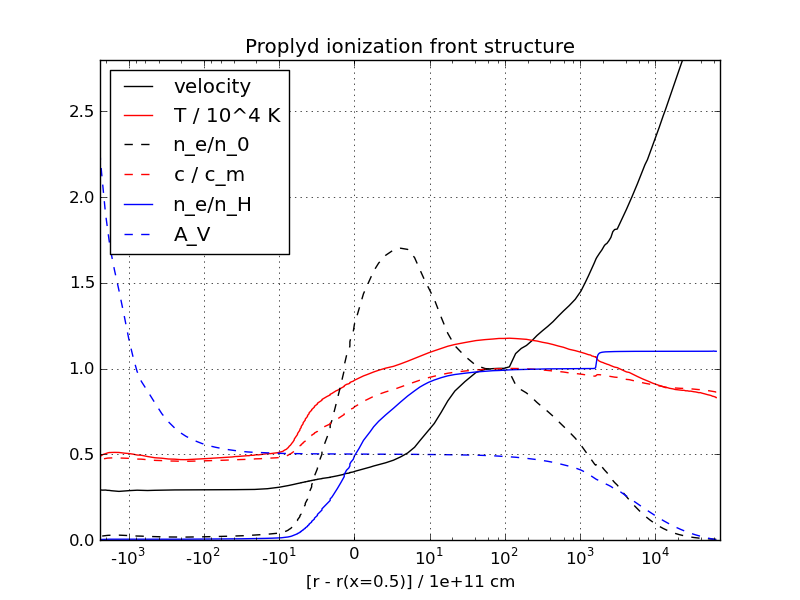
\includegraphics[width=8.5 cm]{ifrac-vs-Rlog.png}
  \caption{1D model structure of several physical properties.} \label{fig:ifrac}
\end{figure}

%--------------------------------------------------------
\subsection{Ionization structure}
\label{sec:ionization}
%--------------------------------------------------------



%--------------------------------------------------------
\subsection{Emissivities}
\label{sec:emi}
%--------------------------------------------------------

All the high ionization lines are all wholly outside the sonic point.

\neii, \ha, \nii and \oii have almost the 90\% of their emission in the supersonic zone and the 10\% in the sub-sonic zone.

\sii is about 70\% outside the sonic point and 30\% inside.

\oi is about 20\% outside and 80\% inside the sonic point.

So if we take into account the full emission of the proplyd, and the sub-sonic zone is not well modelated, the efect of this should be not very important since it is only going to affect two lines. Nevertheless, if we want to compare the model predictions with observations that takes only a little aperture of the proplyd and it is near of the center (near the I-front), the sub-sonic zone will be very important.

There are a clear separation of 3 km/s (about 15\%) between the median velocity of the \oiii 5007 and 4363 lines.

Discutir tambien la diferencia que hay entre la linea auroral y la nebular de \nii para ver la importancia de las desexitaciones colisionales. Una es mas afectada que la otra y por lo tanto conforme vamos a las zonas de mayor densidad la razon entre ellas debe ir cambiando, aumentando de hecho.

%--------------------------------------------------------
\subsection{Aperture and Inclination}
\label{sec:aperture}
%--------------------------------------------------------


%--------------------------------------------------------
\subsection{IR Emission}
\label{sec:IR}
%--------------------------------------------------------


%--------------------------------------------------------
\section{Conclusion}
\label{sec:conclusions}
%--------------------------------------------------------

We will construct Cloudy models of a series of individual radial cuts from the center of the proplyd, at different angles $\theta$ from the proplyd axis.

%--------------------------------------------------------
\section{Acknowledgements}
\label{sec:Acknowledgements}
%--------------------------------------------------------

\bibliographystyle{t}

\bibliography{biblio}

\end{document}
